\subsection{Physical model and hypothesis}

In this section, we look at a control loop with a plant (external state we wish to maintain), a sensor which measures the plant state, a controller and an actuator. The actuator can be \textit{on} or \textit{off}, which gives two different progression modes for the plant. 
The controller sets the actuator \textit{on} or \textit{off} according to the input from the sensor and the settings from an operator.
Said operator can decide to enable or disable control, and can set preferences for the value to maintain the state around. This is summarized in Figure~\ref{plant}. For now, we assume the operator enables the control (no interest otherwise) and doesn't change the settings.

\begin{figure}[ht]
\begin{center}
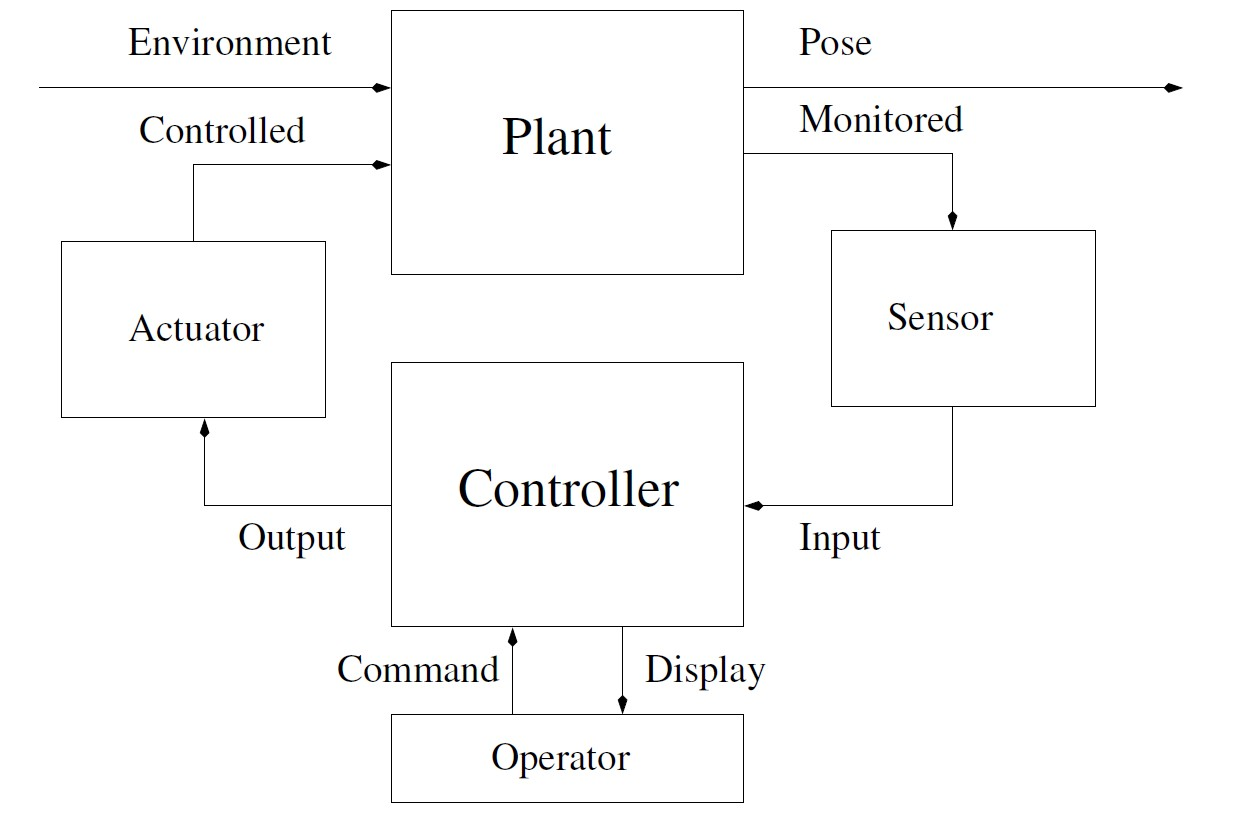
\includegraphics[height=7cm]{plant_controller.jpg}
\caption{The plant controller model}\label{plant}
\end{center}
\end{figure}


We consider the plant state as a real function of the time. The aim for the plant controller is to bring this state between two bounds and to maintain it there. A first example could be a thermostat: we want to maintain a room temperature around a comfortable value by switching a heater \textit{on/off} when needed.
We can also imagine maintaining a correct speed for a vehicle by giving or not power to the engine.

For better comprehension, we will use the vocabulary of the thermostat example in the rest of this section (but the model is actually more general).
We name $\theta (t)$ the temperature at time $t$, and $\tau$ and $\Gamma$ the upper and lower bounds in which we want to maintain the temperature.
We consider that the room leaks energy, and that the heater is powerful enough to increase the room temperature. Typically, while the heater is off, the room temperature decreases with a rate of at most $\mu$, and it increases with a rate of at least $\nu - \mu$ ($\nu > \mu$) while the heater is on. More precisely, considering the temperature is piecewise differentiable,

\[ \left\{ \begin{array}{rcccccll}
0 < & \nu - \mu & < & \dot \theta & < & \Omega   &    &\textrm{If the heater is \textit{on}}\\
    &- \mu    &   < & \dot \theta & < & - \omega & < 0 & \textrm{If the heater is \textit{off}}
\end{array}\right. \]

Assuming the outside temperature is lower than the inside temperature (who needs a heater otherwise?), this model is quite realistic, at least in a reasonable inside temperature range.

To represent real-life devices, we allow the sensor to be slightly inaccurate. Therefore, if the actual temperature is $\theta$, the sensed temperature will be $\sigma$ with 
$\theta - \epsilon \leq \sigma \leq \theta + \epsilon $



\subsection{Controller strategy}

The intuitive way is to set the heater \textit{on} when the temperature is too low, and set it \textit{off} when the temperature is too high. We define two trigger temperatures $\Delta_1$ and $\Delta_2$ with $\tau < \Delta_1 \leq \Delta_2 < \Gamma$. 
When the measured temperature is below $\Delta_1$, the controller switches the heater to \textit{on}, and 
when the measured temperature is above $\Delta_2$, the controller switches the heater to \textit{off}. 
The behavior when the temperature is between $\Delta_1$ and $\Delta_2$ doesn't really matter, so we decide for example to resend previous command.

Of course, we do not use $\tau$ and $\Gamma$ as triggers because of the sensor inaccuracy and because of the potential message latency (see Figure~\ref{trig}).

\begin{figure}
\begin{center}
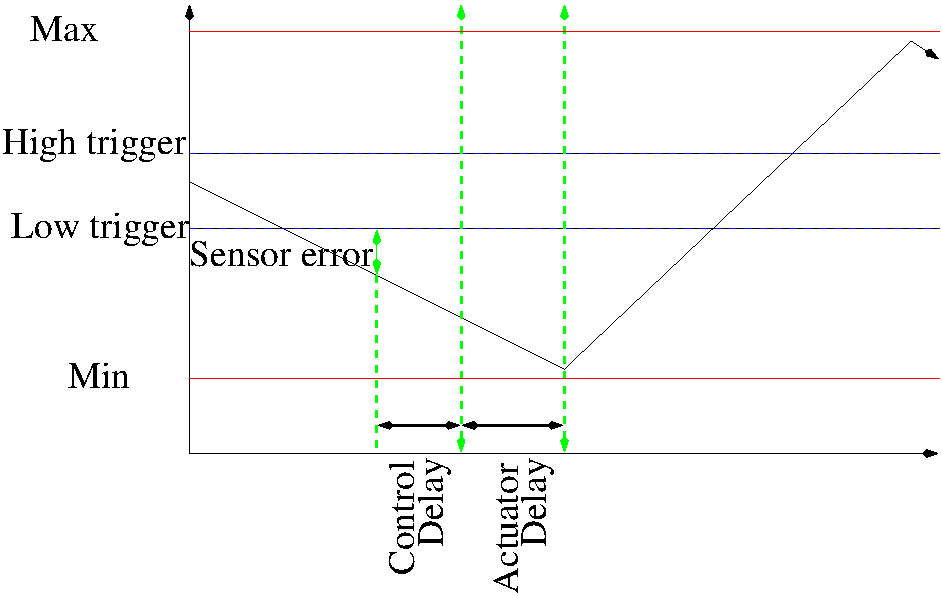
\includegraphics[height=7cm]{thermobehavior.pdf}
\caption{Effect of sensor inaccuracy and control and actuation latencies}\label{trig}
\end{center}
\end{figure}

This strategy could be implemented as follows: The controller keeps a binary setting, initialized to some default value. At each step, if a new message have been received, the controller chooses the most recent one and look at the sensed temperature $\sigma$ inside.
If $\sigma < \Delta_1$, the setting is turned to \textit{on}. If $\sigma > \Delta_2$, the setting is set to \textit{off}. Otherwise, no change is applied to the setting. After this test, the current setting is sent to the actuator.
(using the previous setting also in case no new message have been received is equivalent to use a backup from the previous computation)


\subsection{Correctness proof}\label{MAdef}

To prove correctness of the system, we need to apply this physical model to our logical architecture.
We name $S$, $C$ and $A$ the nodes for the sensor, the controller and the actuator respectively.
We note $s(n)$, $c(n)$ and $a(n)$ the time when their respective nth computation occurs. Let $Input$ and $Output$ be the topics for the sensed temperature and control commands respectively 
(that is, $S$ publishes to $Input$, $C$ subscribes to $Input$ and publish to $Output$, and $A$ subscribes to $Output$). 
Let finally $r_1(n)$ and $r_2(n)$ be the times when the nth message in these topics is delivered.

\vbox{
\begin{defin}\Thmname{Plant controller characteristic time}

For a topic $T$, we note $MA(T)$ some bound for the age of latest available message\footnotemark at each step (given for example by theorem~\ref{maxAge} or theorem~\ref{maxAge2}).

The characteristic time for the plant controller is the quantity
\[ \lambda = MA(Input) + MA(Output) + maxT(A)\]
\end{defin}
}
\footnotetext{$ $ see definition~\ref{ageDef}}

\vbox{
\begin{thm}\Thmname{State stability}\label{control}

Assume $\theta(t) \geq \Delta_1 - \epsilon \geq \tau + \lambda.\mu$ for some time $t$. Then, $\theta(t)$ never drops below $\tau$ after that: \mbox{$\forall t' \geq t, \, \theta(t') > \tau$}

Symmetrically, assume $\theta(t) \leq \Delta_2 + \epsilon\leq \Gamma - \lambda.\Omega$ for some time $t$. Then, $\theta(t)$ never becomes above $\Gamma$ after that: \mbox{$\forall t' \geq t, \, \theta(t') < \Gamma$}
\end{thm}
}

\begin{proof}
Let $t' \leq t$ and $g = glb(\{u \in \mathbb{R}, \, t \leq u \leq t' \textrm{ and } \theta(u) \leq \Delta_1 - \epsilon\})$. By definition, $\theta(g) = \Delta_1 - \epsilon$ and $g < u \leq t' \implies \theta(u) < \Delta_1 - \epsilon$.

Given $\dot{\theta} > -\mu$, if $t' \leq g + \lambda$, the result is proved. Otherwise, we prove $\theta(t') \geq \theta(g + \lambda) > \tau$, because the actuator is always \textit{on} in the time  interval $[g + \lambda, t']$:

Let $u \geq g + \lambda$. The actuator state at time $u$ was set at the latest computation $a(n)$ of $A$.
$a(n+1) \leq a(n) + maxT(A)$ so we have $a(n) > g + MA(Input) + MA(Output)$.
The corresponding command from the thermostat was issued at some $c(k)$ and by definition of $MA(Output)$,
we have $c(k) > g + MA(Input)$. This command was computed by comparing a measured temperature with $\Delta_1$ and $\Delta_2$.
Let $s(l)$ the execution that measured this temperature. We have $s(l) > g$ (by definition of $MA(Input)$), which means $\theta(s(l)) < \Delta_1 - \epsilon$.
Therefore, the sensed temperature was \mbox{$\sigma(s(l)) < \Delta_1$}
\end{proof}

\begin{thm}\Thmname{State convergence}

Assume $\theta(t) < \Delta_1 - \epsilon$. Then we have $\theta(t') \geq \Delta_1 - \epsilon$ for some $t'$ with 
\[t' < t + \lambda + \frac {\Delta_1 - \epsilon - \theta(t) + \lambda.\mu} {\nu - \mu} \]

Symmetrically, assume $\theta(t) > \Delta_2 + \epsilon$. Then we have $\theta(t') \leq \Delta_2 + \epsilon$ for some $t'$ with
\[t' < t + \lambda + \frac {\theta(t) + \lambda.\Omega - \Delta_2 - \epsilon} {\omega} \]
\end{thm}

\begin{proof}
Assume for all $u$ with $t \leq u \leq T = t + \lambda + \frac {\Delta_1 - \epsilon - \theta(t) + \lambda.\mu} {\nu - \mu}$, we have $\theta(u) < \Delta_1 - \epsilon$.
With the same argument as in previous theorem, the heater is always on in the time interval $[t + \lambda, T]$. 

During this interval, the temperature increases at a minimum rate of $\nu - \mu$. Therefore, $\theta(T) > \theta(t + \lambda) + (\Delta_1 - \epsilon - \theta(t) + \lambda.\mu)$. But $\theta(t + \lambda) > \theta(t) - \lambda.\mu$, which leads to a contradiction
\end{proof}






